Every developer writes nested loops now and then.
Many times, nested loops appear compelling and inevitable.
While they may solve our problem, nested loops inflict on a program
unnecessary complexity, obstruct code readability, and bring in `soft duplication'.
The presence of nested loops also thwart optimization at the compiler level.
For these reasons, explicit use of loops at high level programming should be avoided
altogether\cite{data-engineering-avoid-loop}.
Moreover, getting rid of nested loops itself may not seem significant improvement.
The optimizations that are made accessible after getting rid of nested loops dwarfs the improvement
brought about by getting rid of nested loops itself.
Like `Candy Crush Saga' game at certain critical point, a single move may unlock an
avalanche of advantageous moves.


In this section, we are to present a process that coalesces nested loops into single-layered loops,
which we will name as `Nested loop thinning technique'.
For sake of argument, the body of the outer loop is divided into three
sections---\emph{pre-inner-loop} section, \emph{inner-loop} section, and
\emph{post-inner-loop} section---depending on their relative position
in respect to the inner loop (as shown in ~\autoref{fig:segment-for-loop-thinning}).
Cramming the functionalities of nested loops into a single loop is no easy task.
As a price, the process almost always results in one or more of the following:
\begin{itemize}
    \item extra conditional constructs
    \item extra tests added to existing conditional constructs
    \item more dynamic loop pacing
    \item more boundary-condition-handling logic
    \item auxiliary data structure, such as queue or stack
\end{itemize}


\begin{figure}
    \centering
    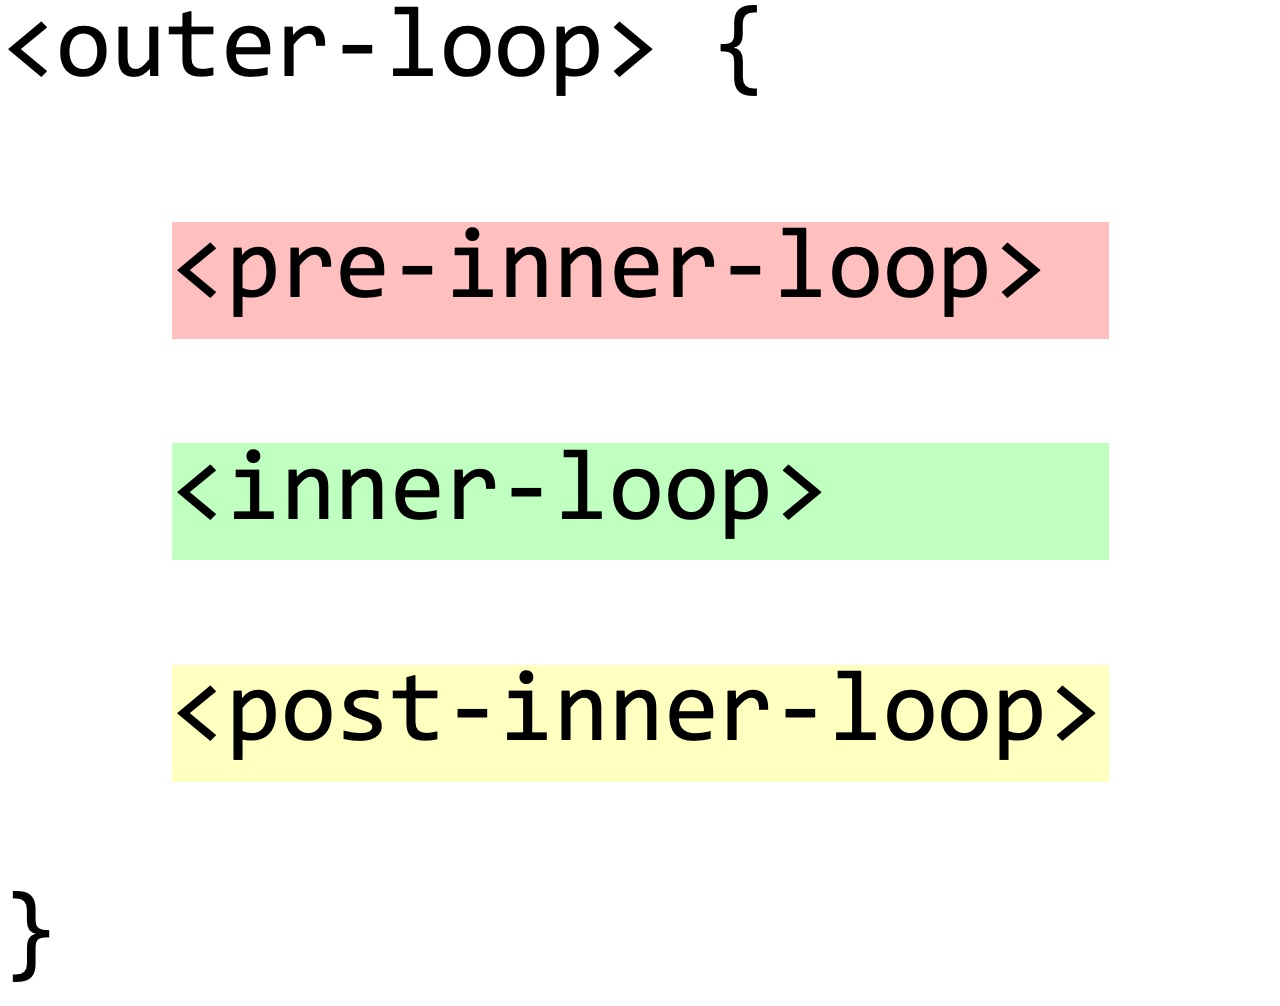
\includegraphics[width=0.4\textwidth]{segment-for-loop-thinning.jpg}
    \caption{\label{fig:segment-for-loop-thinning}
    Sectioning of the body of nested loops:
    \emph{pre-inner-loop} statements, the inner loop itself, and the \emph{post-inner-loop}
    statements.
    Each section receives different treatment during the `nested loop thinning' process.}
\end{figure}


The gist for nested loop thinning process is as follows:
\begin{enumerate}
    \item Preparation stage
    \item Loop rotation to shift around components in the loop body
    \item Reconstruction of loop body using conditionals
\end{enumerate}
But we will go through them one by one.
One will see this pattern again and again for nested loop thinning in practice.


First, some preparatory measures may be taken beforehand
to reduce the friction during the refactor process.
Compound statement is a good example to be dealt with in this step.
Compound statements may get in your way of refactoring for multiple reasons.
The most obvious one is that a compound statement
need to be broken up and sent to different places after refactoring.
State-changing, non-idempotent conditional expressions, such as \code{if (--i < 0)},
are even more lethal because each evaluation of the condition ratchets the state of the loop.
For example,

\begin{minipage}[c]{.3\textwidth}
    \begin{lstlisting}[language=C]
        while (++i < LIMIT);
    \end{lstlisting}
\end{minipage}
\hfill
\begin{minipage}[c]{.3\textwidth}
    shall be expanded to
\end{minipage}
\begin{minipage}[c]{.3\textwidth}
    \lstinputlisting[language=C]{expanded-do-while.java}
\end{minipage}

before the start of loop thinning refactor.
Other types of compound statements, such as \code{if v := a[i]; v < LIMIT}' in Golang, shall be
preprocessed similarly.
Because of the structural similarity between \code{while}-loops and conditionals.
\code{while}-loop readily lends itself to ``nested loop thinning'' process.
For this reason, \code{for}-loop are often converted to \code{while}-loop during preprocessing.


In the second stage, one is to move pre-loop statements, if any, out of the way.
To that end, reverse loop rotation may be used
to unwind the pre-loop statements (see ~\autoref{sec:loop-rotation}).
The second step depends on the inner loop construct.


Finally, it the reconstruction of the loop body using conditional rather than nested loops.
If the inner loop is an unconditional loop as `\code{while True}',
\code{break} statements (or similar) are almost always present and most likely
in a conditional statement somewhere in the loop body unless
it is intended to be a non-typical loop construct.
One should replace the \code{break} statement with the post-inner-loop statements.
The inner loop can then be stripped away.
Otherwise, if the inner loop comes with a non-trivial termination condition,
then the inner loop can be converted to a conditional directly,
\code{while} $\rightarrow$ \code{if},
while the post-inner-loop statements are wrapped away in an \code{else}-clause of it.


Regardless of the venue taken, new conditional statements are inevitably formed or extended
and `cascading conditional construct' are the best way to organize them.
`Cascading conditional construct' consists of ordered sequence of exclusive conditional
statements such as ``\code{if .. elif .. else}''.
For more information, please refer to relevant chapters in Reference ~\cite{Wan:book}.
Throughout the process, one shall pay special attention to execution-path-shunting statements,
such as \code{break} and \code{continue}, if any.


After `nested loop thinning', some cleanup may be performed to comply with convention, code
style, or just for cosmetic reasons.


One disclaimer is that the `nested loop thinning' process does not always prevail.
There are cases where the process is not applicable.
Certain criteria must be met for `nested loop thinning' to be applicable.
First, there must not be intermediate layers, such as
conditional, between the inner and outer loops.
Secondly, execution-path-shunting statements, such as \code{break}, cannot be present in the
pre-inner-loop section.
In what follows, we are going to demonstrate application of `nested loop thinning' technique
on the quicksort algorithms.
